\chapter{z-Transformation}
In diesem Abschnitt werden wir die z-Transformation als ein
wichtiges Werkzeug zur Analyse und zum Verständnis
von LTI-Systemen und ihrer Eigenschaften einführen.
Es werden durch die z-Übertragungsfunktion und dem Pol-Nullstellenplot neue
Beschreibungsformen für LTI-Systeme aufgezeigt.
Insbesondere wird eine Möglichkeit angegeben, um die Stabilität rekursiver LTI-Systeme
zu testen.

\tbd{Beispiel bringen mit Programm (Minihost, Asio4All, pcx) zur Motivation}

\section{Einführung}
Um die Nützlichlkeit dieses Werkzeuges zu untermalen, wollen wir
zunächst von einfachen Beispielen ausgehen.

Angenommen auf ein Sparbuch wird ein bestimmter Geldbetrag $S$
eingezahlt und dieser Betrag wird jährlich mit einem Zins $p$
verzinst. Eine mathematische Darstellung dieses Sachverhalts ergibt sich durch Nutzung des Delta-Impulses gewichtet
mit dem Geldbetrag und einer einfachen Rekursion, wobei ein leeres Konto als Startwert vorliegt. Es gilt also $y(k-1) = 0$.
\begin{equation}\label{eq:ZinsRekursion}
y(k) = (1+p) y(k-1) + S \delta(k)
\end{equation}

Dies ist eine andere Darstellung der Zinseszinsrechenregel. Diese lautet
\begin{equation}
    \mbox{Geld} = S (1+p)^{\mbox{Jahre}}
\end{equation}

Die Anzahl der Jahre ist in \ref{eq:ZinsRekursion} in der Anzahl
der Rekursionen versteckt. Die zweite Form ist eine direkte
Berechnung.
%Diese beiden Möglichkeiten hatten wir auch schon beim
%einführenden Beispiel zur Rekursion gesehen (vergleiche Abschnitt
%\ref{ssec:Rekursion}).

Nun lassen sich aber nicht für alle Rekursionssysteme solche
einfachen direkten Rechenvorschriften angeben. Aber wie ist der mathematische Zusammenhang zwischen den beiden möglichen Lösungen?

In der Rekursionsformel:
\begin{equation}\label{eq:ZinsRekursionWiederholung}
    y(k) = (1+p) y(k-1) + S \delta(k)
\end{equation}
ergibt sich durch Variablensubstitution $c = 1+p$.
\begin{equation}\label{eq:ZinsRekursionMitc}
    y(k) = c y(k-1) + S \delta(k)
\end{equation}
Diese Form wird jetzt auf beiden Seiten mit der Summe $\sum_{k =
-\infty}^{\infty}z^{-k}$ multipliziert. Ein Schritt der
mathematisch erlaubt ist, da er auf beiden Seiten des
Gleichungssystems durchgeführt wird.
\begin{equation}
\sum_{k = -\infty}^{\infty} y(k) z^{-k} = \underbrace{c \sum_{k =
-\infty}^{\infty} y(k-1) z^{-k}}_{\mbox{1. Summand}} +
\underbrace{S \sum_{k = -\infty}^{\infty} \delta(k)
z^{-k}}_{\mbox{2. Summand}}
\end{equation}
Mit Hilfe der abkürzenden Schreibweise 
\begin{equation}\label{eq:Def:zTrafo}
Y(z) = \sum_{k = -\infty}^{\infty} y(k) z^{-k} .
\end{equation}
ergibt sich bei dem 2. Summanden nur ein Element der Summe den Wert
$S$, da die $\delta$-Folge nur bei $k = 0$ einen Wert ungleich
Null hat.

Zusätzlich kann der 1. Summand durch eine
Variablensubstitution $k' = k-1$ umgeformt werden.
\begin{equation}\label{eq:zTrafo:Example1Subst}
    c \sum_{k =
-\infty}^{\infty} y(k-1) z^{-k} = c \sum_{k' = -\infty}^{\infty}
y(k') z^{-k'-1} =c z^{-1}\sum_{k' = -\infty}^{\infty} y(k')
z^{-k'}=c z^{-1} Y(z)
\end{equation}

Somit ergibt sich
\begin{equation}\label{eq:zTrafo:Example1}
    Y(z) = c z^{-1} Y(z) + S .
\end{equation}
Umgestellt folgt
\begin{equation}\label{eq:ztrafo:Example1:zLoesung}
    Y(z) = \frac{S}{1-c z^{-1}} .
\end{equation}

Um zur Lösung für das Ausgangssignal zu kommen, wird die Summenformel für eine geometrische Reihe eingeführt.
\begin{equation}\label{eq:Def:geometrischeReihe}
    \sum_{k = 0}^{\infty} q^k = \frac{1}{1-q}  \quad \mbox{wenn} \quad
    |q|<1
\end{equation}

Für Gleichung \ref{eq:ztrafo:Example1:zLoesung} ergibt sich also
\begin{equation}\label{eq:zTrafo:Example1:kLoesung1}
    \frac{S}{1-c z^{-1}} = S \sum_{k = 0}^{\infty} (c z^{-1})^k = S \sum_{k = 0}^{\infty} c^k z^{-k}
\end{equation}

Vergleicht man diese Lösung mit \ref{eq:Def:zTrafo} so ergibt sich
\begin{equation}\label{eq:zTrafo:Example1:kLoesung2}
    y(k) = \bigg\{ \begin{array}{lcc}
      S c^k & & k \geq 0\\
        0  & & k<0
    \end{array} = S(1+p)^k \gamma(k)
\end{equation}
mit $\gamma(k)$ als Sprungfolge (siehe Gl.
\ref{eq:Def:Sprungfolge}).

Dies entspricht der vorher bekannten Lösung für die
Zinseszinsformel.


\section{Definition}
Für eine verkürzte
Schreibweise wird für die z-Transformation folgendes Symbol eingeführt
\begin{equation}\label{eq:Def:Ztrafo}
    \ZT{ \cdot }= \sum_{k = -\infty}^{\infty} (\cdot) z^{-k} \Mit z \in \mathbb{C}
\end{equation}

Es gilt also
\begin{equation}\label{eq:yExample}
    Y(z) =\ZT{y(k)}
\end{equation}
Die Rechenvorschrift führt dazu, dass die diskrete Eingangsfolge
$y(k)$ abgebildet wird auf eine komplexe Ebene. Man spricht
deshalb auch von Zeitbereichsdarstellung und
Bildbereichdarstellung. Um die Korrespondenz zu symbolisieren wird
häufig der sog. ''Transformationsknochen'' verwendet.
\begin{itemize}
    \item Hintransformation: $y(k)\HinTrans Y(z)$ oder bei Gleichungsabfolgen $\HinTransV$
    \item Rücktransformation: $Y(z) \RueckTrans y(k)$ oder $\RueckTransV$
\end{itemize}

Damit eine z-Transformation gültig ist, muss zusätzlich gelten,
dass die Summe in Gl. \ref{eq:Def:Ztrafo} kleiner unendlich ist.
Dies ist für alle endlichen Folgen gegeben, wenn
keiner der Folgenwerte unendlich ist. Bei unendlichen Folgen ist dies
nicht immer gewährleistet.und hängt auch
direkt von der Wahl des $z$ ab. Deshalb gehört zu einer
vollständigen Beschreibung der z-Transformation auch immer die
Bereichsangabe von $z$ in der die Summe konvergiert. Man spricht deshalb vom sogenannten
Konvergenzgebiet {\em Region of Convergence}.
Zur Beschreibung des Konvergenzgebietes reichen die
Angaben der Radien $r = |z|$ der komplexen Zahlen aus. Für das
Konvergenzgebiet ergibt sich entweder das Gebiet inner- oder außerhalb einer
Kreisfläche oder das Gebiet hat die Form eines Kreisringes in der z-Ebene.

\begin{figure}[H]
\begin{center}
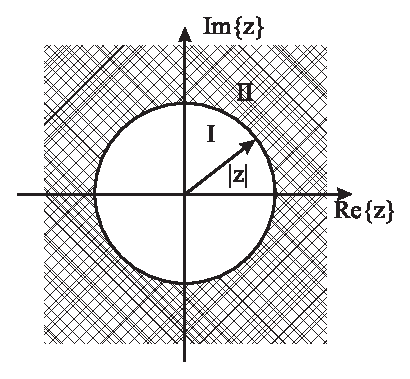
\includegraphics[width = 8cm]{psZ/ROC_Kausal}
\caption{\label{pic:ROC_Kausal} Veranschaulichung des Konvergenzgebietes
bei der z-Transformation. In diesem Beispiel für eine kausale Folge (ROC außerhalb).}
\end{center}
\end{figure}

\begin{example}
%\begin{minipage} {14cm}
\label{Bsp:z_TrafoUndROC} Betrachtet man die kausale Folge (siehe Abbildung \ref{pic:zFolgnPic}a)
(Sie entspricht dem Sparbuchbeispiel mit einem Startkapital von
0.5 und 50\% Kontokosten (Also einer ziemlich schlechten Geldanlage).)
\begin{eqnarray} \label{eq:BspKausaleFolge}
    x(k) &=& [0.5 \:\: 0.5^2 \:\: 0.5^3 \:\: \cdots \:\: 0.5^k]\\
         & = & 0.5^k \gamma(k) \qquad \fuer k \geq 0 ,
\end{eqnarray}
so ergibt sich die z-Transformierte als
\begin{equation}
    X(z) = \sum_{k = -\infty}^{\infty} 0.5^k \gamma(k)z^{-k}
    = \sum_{k = 0}^{\infty} 0.5^k z^{-k} =
    \sum_{k = 0}^{\infty} (0.5z^{-1})^{k}
\end{equation}
bzw. mit der Umformung durch die geometrische Reihe
\begin{equation}
    X(z) = \frac{1}{1-0.5z^{-1}} = \frac{z}{z-0.5},
\end{equation}
wobei das Konvergenzkriterium der geometrischen Reihe zusätzlich
\begin{equation}\nonumber
    |0.5z^{-1}| = \frac{0.5}{z} < 1 \qquad \Rightarrow \qquad |z| > 0.5
\end{equation}
fordert.

\begin{figure}[H]
\begin{center}
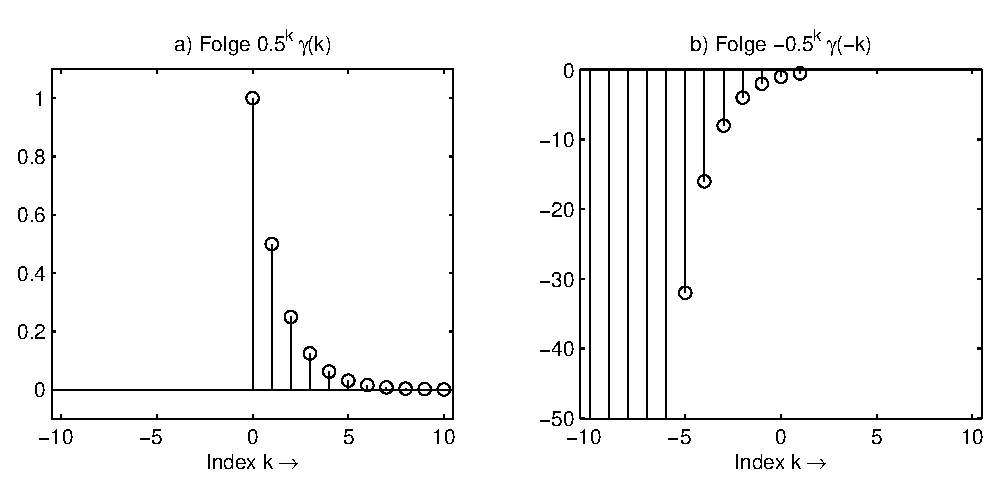
\includegraphics[width = 10cm]{psZ/zFolgenPic}
\caption{\label{pic:zFolgnPic} a) kausale Folge $0.5^k \gamma(k)$ für $ k \geq 0 $
und b) nicht-kausale Folge $-0.5^k \gamma(-k-1)$ für $k < 0$.}
\end{center}
\end{figure}

Im folgenden soll nun eine sehr ähnlichen Folge, nämlich
dem nicht-kausalen, negativen äquivalent zu \ref{eq:BspKausaleFolge}
\begin{equation}\nonumber
    x(k) = -0.5^k \gamma(-k-1) \qquad \fuer k < 0
\end{equation}
betrachtet werden (siehe Abbildung \ref{pic:zFolgnPic}b).
Berechnet man die z-Transformierte ergibt sich mit einer Variablensubstitution $k = -m$
\begin{eqnarray}\nonumber
    X(z) &=& - \sum_{k = -\infty}^{-1} 0.5^k z^{-k} \\
    & = &- \sum_{k = -\infty}^{-1} (0.5^{-1}z)^{-k} \\
    & = &- \sum_{m = 1}^{\infty} (0.5^{-1}z)^{m}
\end{eqnarray}
Nutzt man jetzt eine alternative Formulierung der unendlichen geometrischen
Reihe
\begin{equation}\nonumber
    \sum_{m = 1}^{\infty} x^m = \frac{x}{1-x}
\end{equation}
so ergibt sich
\begin{equation}\nonumber
    X(z) = - \frac{0.5^{-1}z}{1-0.5^{-1}z} = \frac{z}{z-0.5}
\end{equation}
Wir erhalten also die gleiche z-Transformation für unterschiedliche Folgen, wobei aber
die Konvergenz der geometrischen Reihe für die anti-kausale Folge ein Konverzgebiet
\begin{equation}\nonumber
    |z| < 0.5
\end{equation}
fordert. Abbildung \ref{pic:ROC_AntiKausal} zeigt das dazugehörige Konvergenzgebiet
in der z-Ebene.
Man erkennt somit, warum eine Angabe des ROC bei der z-Transformation notwendig ist, um eine
eindeutige Berechnung und Zuordnung zu gewährleisten.
\begin{figure}[H]
\begin{center}
\includegraphics[width = 8cm]{psZ/ROC_AntiKausal}
\caption{\label{pic:ROC_AntiKausal} Veranschaulichung des Konvergenzgebietes
bei der z-Transformation. In diesem Beispiel für eine anti-kausale Folge (ROC innerhalb) mit
$|z| < 0.5$.}
\end{center}
\end{figure}
%\addtolength{\hoffset}{-3cm}
\hspace{0.1mm}
\end{example}
%\end{minipage}

\section{Rechenregeln}
Die z-Transformation erleichtert das
Rechnen von Differenzengleichungen. Wir werden deshalb im weiteren
einige häufig verwendete Rechenregeln und Korrespondenzen
einführen.

\subsection{Linearität}
Die z-Transformation ist eine lineare Transformation. Es gilt:
\begin{equation}\label{eq:zTrafo:Linearitaet}
  a_1 x_1(k) + a_2 x_2(k) \HinTrans a_1 X_1(z) + a_2 X_2(z)
\end{equation}

\subsection{Verschiebung}
Die zeitliche Verschiebung der diskreten Folge haben wir bereits
in den Beispielen ausgiebig verwendet. Es gilt:
\begin{equation}\label{eq:zTrafo:Verschiebungssatz}
    \mathcal{Z}\{y(k-k_0)\} = z^{-k_0} Y(z)
\end{equation}

\section{Rück-Transformation}
Wir haben gesehen, dass die z-Transformation eine diskrete Folge
in eine kontinuierliche komplexe Ebene transformiert. In den
Beispielen hatten wir es für die Rücktransformation in den
Zeitbereich stets mit einfachen gebrochen rationalen Funktionen zu
tun, die direkt auf eine bestimmte Folge führten. Dies ist nicht
immer möglich. Die allgemeinste Version der z-Rücktransformation
ist durch das Umlaufintegral
\begin{equation}\label{eq:zRuek:Def}
    x(k) = \oint_C X(z) z^{k-1} dz
\end{equation}
gegeben. Dies bedeutet wir umlaufen die komplexe Ebene auf dem
Kreis C im mathematisch positiven Sinn (Gegenuhrzeigersinn) und
integrieren die eingeschlossene Fläche. Dies ist nicht immer
möglich. Ob die Möglichkeit besteht hängt direkt davon ab, wie das
Konvergenzgebiet definiert ist. Auf die  explizite Behandlung der
Thematik wird hier nicht eingegangen, statt dessen wird auf \cite{OS99}
verwiesen, die Stichworte, die man sich im
Zusammenhang mit der Rücktransformation merken sollte sind:
Cauchy-Integral, Laurent-Reihe, Residuensatz.

In vielen Fällen kann auf die Lösung des Integrals verzichtet
werden. Statt dessen sind häufig Lösungen über
Partialbruchzerlegung (siehe Beispiele) und/oder
Korrespondenztabellen möglich


\subsection{Korrespondenztabelle}

Viele Systeme und Signale lassen sich auf einfache Grundformen
zurückführen. Für diese Grundformen kann für die Hin- und
Rücktransformation folgende Tabelle verwendet werden.

\begin{tabular}{|c|c|c|}
  \hline
  % after \\: \hline or \cline{col1-col2} \cline{col3-col4} ...
  Zeitbereich $y(k)$ & Bildbereich $Y(z) = \ZT{y(k)}$ & Konvergenzgebiet \\
  \hline
  $\delta(k)$     & 1                                 & $\forall z$\\
  $\gamma{k}$     & $\frac{z}{z-1} = \frac{1}{1-z^{-1}} $ & $|z|>1$ \\
  $k \gamma(k)$   & $\frac{z}{(z-1)^2}$               & $|z|>1$\\
  $e^{-\alpha k}\gamma (k)$ & $\frac{z}{z-e^{-\alpha}}$  & $|z|>e^{-\alpha}$\\
  $\alpha^k \gamma (k)$ & $\frac{z}{z-\alpha}$ & $|z| > \alpha$ \\
  $\cos(\omega_0 k)$ & $\frac{1-z^{-1} \cos(\omega_0)}{1-z^{-1} 2\cos(\omega_0)+z^{-2}}$ & $|z|>1$\\
  \hline
\end{tabular}

Eine Beschreibung von LTI-Systemen kann wie im letzten Abschnitt gezeigt
über Differenzengleichungen erfolgen.
Die z-Transformation und Rücktransformation solcher Systeme sind besonders
gut über die Korrespondenztabellen zu lösen:
\hspace*{1cm}

\begin{example}
LTI-Systeme\\
Wie lautet die z-Transformierte für die folgende Differenzengleichung
\[
    y(k) = 0.2y(k-1) - y(k-3) + x(k) + 1.2x(k-1) - 3.2 x(k-2)
\]
Entscheidend ist, dass nur einfache Verzögerungen $k_0$ auftreten, die in der z-Ebene
durch $z^{-k_0}$ dargestellt werden.
Es ergibt sich mit der Eigenschaft der Linearität:
\[
    Y(z) = 0.2Y(z) z^{-1} - Y(z) z^{-3} + X(z) + 1.2X(z) z^{-1} - 3.2X(z) z^{-2}
\]
\end{example}

\section{Systemfunktion\label{sec:Systemfunktion}}
Bei den zur Einführung verwendeten Beispielen wurden sehr einfache
Eingangsfolgen für $x(k)$ verwendet. Man könnte das
Sparbuch-Beispiel aber auch erweitern und annehmen, dass pro Jahr
eine nicht näher definierte Summe zusätzlich aufs Konto eingezahlt
wird. Die rekursive Formulierung für den Ausgang sehe dann wie
folgt aus
\begin{equation}\label{eq:example3:Eingang}
    y(k) = (1+p) y(k-1) + x(k)
\end{equation}
Wenn wir diese Gleichung mit der Definition \ref{eq:Def:Ztrafo} in
den z-Bereich transformieren erhalten wir
\begin{equation}\label{eq:eaxample3:zLoesung}
    Y(z) = (1+p)z^{-1} Y(z) + X(z)
\end{equation}
Dies ergibt umgeformt
\begin{equation}\label{eq:eaxample3:zLoesung2}
    Y(z) = \frac{X(z)}{1-(1+p)z^{-1}}
\end{equation}

Teilen wir diese Lösung durch $X(z)$ erhalten wir auf der rechten
Seite der Gleichung den Anteil, der unabhängig vom Eingangssignal
ist und nur das System repräsentiert. Wir kürzen zusätzlich den
Bruch $Y(z)/X(z)$ mit $H(z)$ ab.
\begin{equation}\label{eq:example3:Systemfunktion}
    H(z) = \frac{Y(z)}{X(z)} = \frac{1}{1-(1+p)z^{-1}}
\end{equation}
Die Funktion $H(z)$ wird z-Übertragungsfunktion genannt und
beschreibt ein LTI-System vollständig. Eine andere vollständige
Beschreibung eines LTI-Systems unabhängig vom Eingangssignal war
die Impulsantwort $h(k)$ eines Systems. Beide Darstellungsarten
sind durch die z-Transformation miteinander verbunden. Es gilt:
\begin{equation}\label{eq:Def:UbertragFunktion}
    \ZT{h(k)} = H(z)
\end{equation}
\wichtig{Die z-Transformation der Impulsantwort $h(k)$ ist die Systemfunktion $H(z)$}
\begin{example}
z-Übertragungsfunktion\\
Die z-Transformierte aus dem vorherigen Beispiel war gegeben durch
\[
    Y(z) = 0.2Y(z) z^{-1} - Y(z) z^{-3} + X(z) + 1.2X(z) z^{-1} - 3.2X(z) z^{-2}
\]
die z-Übertragungsfunktion ergibt sich durch wenige
Umformungsschritte
\begin{eqnarray}\nonumber
    Y(z)- 0.2Y(z) z^{-1} + Y(z) z^{-3} & = &  X(z) + 1.2X(z) z^{-1} - 3.2X(z) z^{-2}\\\nonumber
    Y(z) \left(1-0.2z^{-1} + z^{-3} \right) &=& X(z) \left(1 +1.2z^{-1} - 3.2 z^{-2} \right)\\
    H(z) = \frac{Y(z)}{X(z)} &= & \frac{1 +1.2z^{-1} - 3.2 z^{-2}}{1-0.2z^{-1} + z^{-3}}
\end{eqnarray}
\end{example}

Die Verknüpfung von $h(k)$ und dem Eingangssignal $x(k)$ zum
Ausgangssignal $y(k)$ erfolgte im Zeitbereich über die Faltung.
Bei der z-Übertragungsfunktion ist die Verknüpfung von Eingang und
Ausgang durch die Multiplikation gegeben. Es gilt also
\begin{equation}\label{eq:zTrafo:FaltungMulti}
    \ZT{a(k)\ast b(k)} = A(z) B(z)
\end{equation}
Damit haben wir eine Möglichkeit gefunden die eher aufwendige
Faltungsumme mit Hilfe der z-Transformation in eine einfache
Multiplikation im z-Bereich zu überführen. Das Ausgangssignal
erhält man abschließend durch die inverse z-Transformation des
Ausgangssignals $Y(z)$. Dieser Lösungsweg ist in Abbildung \ref{pic:SchemaZLoesungFaltung}
zur Verdeutlichung schematisch gezeigt.

\begin{figure}[H]
\begin{center}
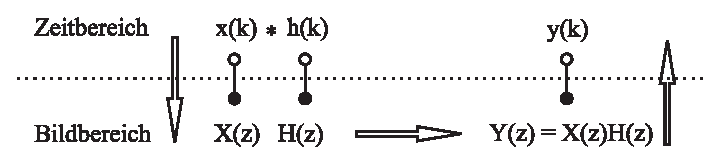
\includegraphics[width = 10cm]{psZ/SchematischezLoesungFaltung}
\caption{\label{pic:SchemaZLoesungFaltung} Schematische Darstellung zur Berechnung
der Faltungssumme mit Hilfe der z-Transformation.}
\end{center}
\end{figure}

\begin{example}
Das System ist durch
\[
    y(k) = x(k) -2x(k-1) + x(k-2)
\]
gegeben. Die z-Transformation führt auf eine z-Übertragungsfunktion
\[
    H(z) = 1-2z^{-1} + z^{-2}
\]
Für die Eingangsfolge:
\[
    x(k) = \delta(k) + 2\delta(k-1)  + 3\delta(k-2)  + 4\delta(k-3)  + 5\delta(k-4)
\]
ergibt sich die z-Transformierte zu
\[
X(z) = 1 + 2z^{-1} + 3z^{-2}+ 4z^{-3}+ 5z^{-4}
\]
Eine Polynommultiplikation führt zu der Ausgangs-z-Funktion
\[
Y(z) = X(z)H(z) = 1 -6 z^{-5} + 5 z^{-6}
\]
Damit ergibt sich für die Ausgangsfolge
\[
    y(k) = [1 \:\: 0 \:\: 0 \:\: 0 \:\: 0 \:\: -6 \:\: 5]
\]
bzw.
\[
    y(k) = \delta(k) - 6 \delta(k-5) + 5 \delta(k-6)
\]
\end{example}

\wichtig{Die Faltung wird in der z-Ebene zu einer Multiplikation}

\section{Pol-Nullstellenplan}
Nachdem die Äquivalenz der Impulsantwort mit der
z-Übertragungsfunktion $H(z)$ bekannt ist, ist es möglich, Systeme
besser zu analysieren. Dazu schauen wir uns zunächst die typische
Übertragungsfunktion an.
\begin{equation}\label{eq:Uebertragungsfunktion}
 H(z) = \frac{b_0 + b_1z^{-1} + b_2z^{-2}+ \cdots b_M z^{-M}
    }{1 + a_1z^{-1} + a_2z^{-2}+ \cdots a_N z^{-N}}
    = \frac{\displaystyle \sum_{i=0}^M b_iz^{-i}}
    {\displaystyle \sum_{i=0}^N a_i z^{-i}} \Mit a_0 = 1
\end{equation}
Wir nehmen an, dass der Zählergrad $M$ kleiner oder gleich dem
Nennergrad $N$ ist. Dies ist gleichbedeutend mit der Annahme, dass
es sich um ein kausales System handelt\footnote{Würde gelten $M>N$
könnte man durch Polynomdivision eine Übertragungsfunktion
erhalten, die aus einem simplen Polynom und einer gebrochen
rationalen Funktion mit $M\leq N$ besteht, wobei das Polynom ein
Polynom in $z$ und nicht in $z^{-1}$ wäre und somit bei einer
z-Rücktransformation auf einen nicht-kausalen Anteil führen
würde.}. Die Ordnung des Systems wird unter dieser Annahme durch $N$
angegeben. Im allgemeinen Fall definiert das Maximum von $N$ und $M$
die Ordnung des Systems.

Die gebrochen rationale Funktion können wir auch in der
äquivalenten Produktform schreiben, wenn uns alle Nullstellen, des
Zähler- und Nennerpolynoms bekannt sind. Wir werden für die
Nullstellen des Nenners ab jetzt den Begriff Polstellen bzw. Pol
verwenden, da an diesen Punkten, die Übertragungsfunktion
unendlich wird.

\begin{eqnarray}\label{eq:Uebertragungsfunktion:Produktdarstellung}
 H(z)
 & = & b_0 \frac{(z-n_0)(z-n_1)\cdots(z-n_{M-1})}{(z-p_0)(z-p_1)\cdots(z-p_{N-1})}\\
 & = & b_0 \frac{\displaystyle \prod_{i = 0}^{M-1}(z-n_i)}
 {\displaystyle \prod_{i = 0}^{N-1}(z-p_i)}
 \end{eqnarray}

Für reelle Koeffizienten $b_i$ und $a_i$ ergeben sich dabei immer
nur reelle Nullstellen oder konjugiert komplexe Paare.

\begin{example}
\begin{eqnarray}\nonumber
    H(z) & = & \frac{3+6z^{-1}+3z^{-2}}{1.0000   -1.7119 z^{-1} +   0.8100
    z^{-2}}\\\nonumber
    &=& 3\frac{(z+1)(z+1)}{(z-0.8560 - 0.2781j)(z-0.8560 +
    0.2781j)}\\\nonumber
    &=& 3\frac{(z+1)^2}{(z-0.9e^{j\frac{\pi}{10}})(z-0.9e^{-j\frac{\pi}{10}})}
\end{eqnarray}
\end{example}

Um bestimmte Eigenschaften zu verdeutlichen ist es oft sinnvoll,
die Pole und Nullstellen in der komplexen Ebene einzuzeichnen.
Dabei werden Nullstellen durch ein o und Pole durch ein x
markiert. Für das Beispiel ergibt sich der folgende
Pol-Nullstellenplan, wobei ein eventuell vorhandener Skalierungsfaktor $b_0$
nicht berücksichtige wird. Der Pol- Nullstellenplan ist deshalb keine
vollständige Beschreibung eines LTI-Systems.
\begin{figure}[H]
\begin{center}
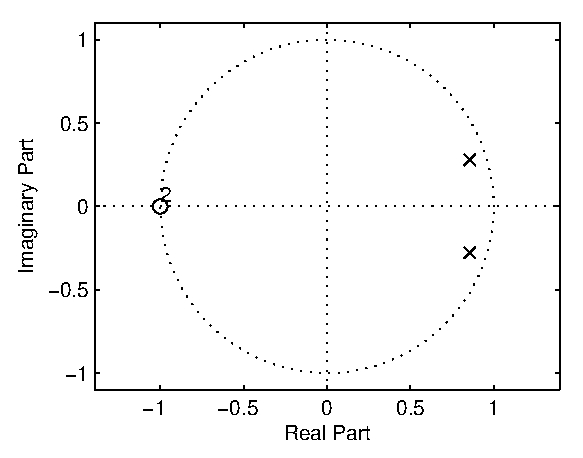
\includegraphics{psZ/PolNullstellenplan}
\caption{\label{pic:bspPolnullstellenplan}Pole und Nullstellen in
der komplexen Ebene.}
\end{center}
\end{figure}
Mehrfachnullstellen (oder auch Pole) werden durch eine zusätzliche
Zahl gekennzeichnet, hier die zwei für die doppelte Nullstelle bei
$z = -1$. Weiterhin ist der sog. Einheitskreis zu sehen, der den
Radius eins markiert und eine besondere Bedeutung hat, auf die wir
noch zu sprechen kommen.

Zur Verdeutlichung der Auswirkungen von Polen und Nullstellen
in der komplexen Ebene ist in Abbildung \ref{pic:PolNullstellenAuswirkung}
der Betrag der Übertragungsfunktion in Abhängigkeit vom Real und Imaginärteil
für das eben verwendete Beispiel gezeigt (Die Darstellung erfolgt logarithmisch.).
Zur Orientierung ist zusätzlich der Einheitskreis eingezeichnet.

\begin{figure}[H]
\begin{center}
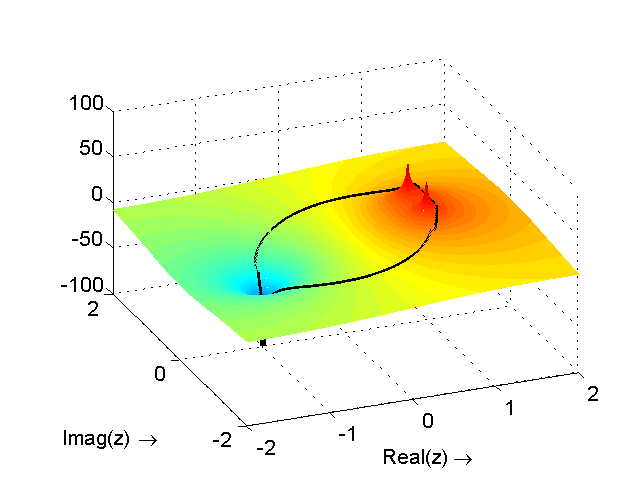
\includegraphics{psZ/PolNullstellenHz}
\caption{\label{pic:PolNullstellenAuswirkung}Übertragungsfunktion in der komplexen Ebene.}
\end{center}
\end{figure}

Der Einfluss der
beide Extremstellen auf den Betrag der Übertragungsfunktion ist auf der ganzen z-Ebene sichtbar.
Man erkennt sehr deutlich, wie die Pole zu einem unendlichen Betrag führen,
während die doppelte Nullstelle den Betrag zu Null werden lässt.

Welche Auswirkungen haben nun Polstellen auf die
Systemeigenschaften und insbesondere auf das Verhalten im
Zeitbereich. Grundsätzlich lassen sich die komplexen Pole immer
auch in der Polarschreibweise (Radius und Phase) angeben.

Betrachten wir jetzt ein System mit nur einem Pol (komplexwertiges
System)
\begin{equation}\label{eq:zTrafo:ErklaerungPolLage}
    H(z) = \frac{1}{1-re^{j\varphi}z^{-1}}
\end{equation}
Zurücktransfomiert in den Zeitbereich ergibt sich mit Hilfe der
Korrespondenztabelle
\begin{equation}\label{eq:zTrafo:ErklaerungPollageZeitbereich}
    h(k) = \gamma(k) r^k e^{j\varphi k}
\end{equation}
Interpretiert man Gleichung
\ref{eq:zTrafo:ErklaerungPollageZeitbereich} so ist zu erkennen,
dass die Impulsantwort aus einer komplexen Schwingung
($e^{j\varphi k}$) und einem Faktor besteht, der die Amplitude
ändert. Dieser Amplitudenfaktor wird als Einhüllende der komplexen
Schwingung bezeichnet. Die Frequenz der Schwingung ist durch den
Polwinkel $\varphi$ definiert und die Form der Einhüllenden durch
den Radius $r$. Für $r<1$ ergibt sich eine gedämpfte
Exponentialfunktion. Bei $r=1$ ist die komplexe Schwingung
ungedämpft und bei $r>1$ handelt es sich um eine aufklingende,
also mit der Zeit stärker werdende Schwingung.

Dies ist in der Abbildung \ref{pic:bspPollagen} nochmals
verdeutlicht. Die Pollage a) ist ein Pol auf der reellen Ache mit
einem Radius von $r = 0.96$\footnote{Die eingezeichneten Pollagen
sind zur Verdeutlichung skaliert.}. Die dazugehörige Schwingung
ist eine abklingende Exponentialfunktion ohne Schwingungsanteil.
Ist der Radius größer
eins (b) $r= 1.01$) ergibt sich eine aufklingende
Exponentialfunktion. Verschiebt man den Pol auf dem Radius $r=
0.96$ auf einen Polwinkel $\varphi = \pi/10$, so ergibt sich eine
exponentiell abklingende Schwingung (siehe c)). Bei einem Radius
größer eins, eine aufklingende Schwingung (d). Die Drehung ist bei
$\varphi = 3\pi / 4$ kaum noch zu erkennen (e), während die
Frequenz $\varphi = \pi$ erneut zu einer reellen Folge führt mit
wechselndem Vorzeichen. Der Radius entscheidet über das
Abklingverhalten (g,f). Die Drehrichtung wird durch die Pollage in
der oberen oder unteren Halbebene angegeben.

\begin{figure}[H]
\begin{center}
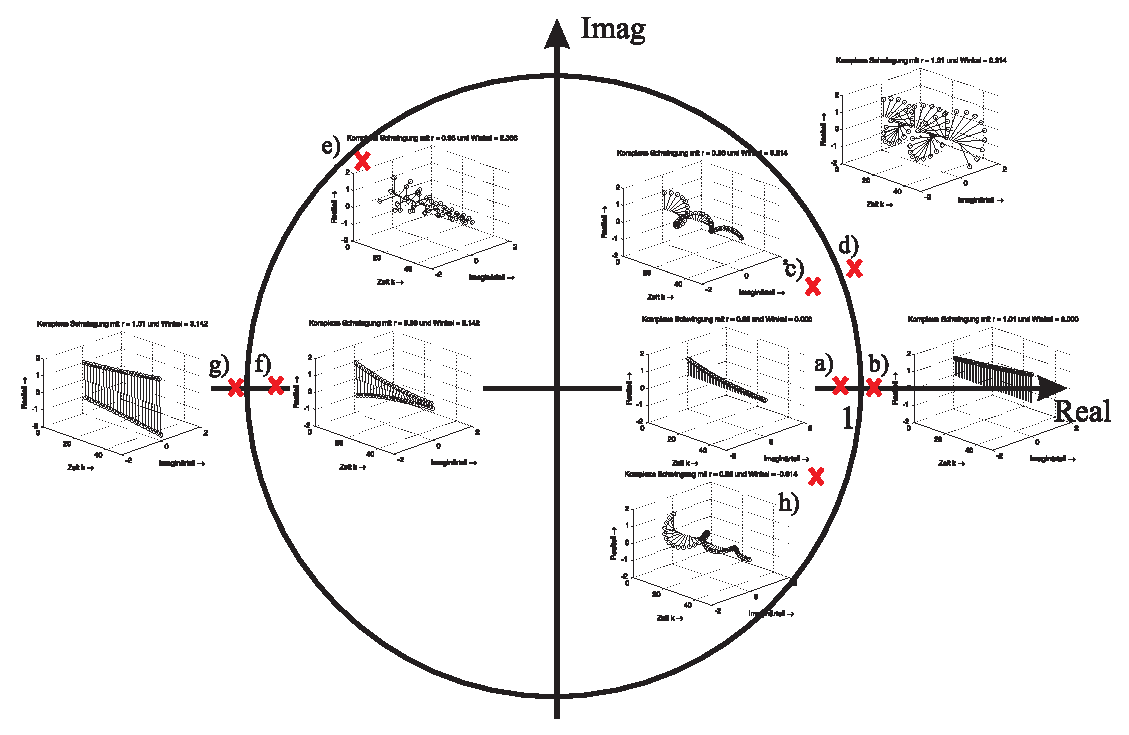
\includegraphics[width = 16cm]{psZ/PolLagen}
\caption{\label{pic:bspPollagen}Mögliche Pollagen und die
dazugehörigen komplexen Schwingungen im Zeitbereich (angelehnt an \cite{girod2013einfuhrung}).}
\end{center}
\end{figure}

Bei konjugiert komplexen Polpaaren heben sich durch die
gegensinnigen Drehrichtungen die Imaginäranteile auf und die
Impulsantwort $h(k)$ ist rein reellwertig. Die ausgebildeten
Schwingungen entsprechen gedämpften oder aufklingenden
Cosinusfunktionen der Frequenz $\varphi$.

Es gilt für
konjugiert ($^{\ast}$) komplexe Polpaare:
\begin{equation}
    \frac{Az}{z-a} + \frac{A^{\ast}z}{z-a^{\ast}} \RueckTrans 2|A||a|^k\cos(arg\{a\}k + arg\{A\})\gamma(k)
\end{equation}
$arg\{x\}$ ist das Argument (Winkel) von der komplexen Zahl $x$.

\begin{example}
Ausgehend von dem System
\[
    H(z) = \frac{z^2}{(z-0.9e^{j\frac{\pi}{10}})(z-0.9e^{-j\frac{\pi}{10}})}
\]
ergibt sich für die Aufspaltung
\[
    H(z) = \frac{Az}{z-0.9e^{j\frac{\pi}{10}}} + \frac{A^{\ast}z}{z-0.9e^{-j\frac{\pi}{10}}}
\]
mit
\begin{eqnarray}
    A &=& (z-0.9e^{j\frac{\pi}{10}})\widetilde{H}(z)\Bigg|_{z = 0.9e^{j\frac{\pi}{10}}}\\
    & = & \frac{z}{z-0.9e^{-j\frac{\pi}{10}}}\Bigg|_{z = 0.9e^{j\frac{\pi}{10}}}\\
    & = & \frac{0.9e^{j\frac{\pi}{10}}}{0.9e^{j\frac{\pi}{10}}-0.9e^{-j\frac{\pi}{10}}}\\
    & = & -j\frac{e^{j\frac{\pi}{10}}}{2\sin \frac{\pi}{10}}
\end{eqnarray}
Die Impulsantwort ist also durch
\[
    h(k) = 2\cdot 1.618 \cdot 0.9^k \cos\left(\frac{\pi}{10}k +\left(-\frac{\pi}{2} + \frac{\pi}{10}\right)\right)\gamma(k)
\]
gegeben und wird in Abbildung \ref{pic:BspKonjKomplexPol} bis $k = 49$ gezeigt.
\begin{figure}[H]
\begin{center}
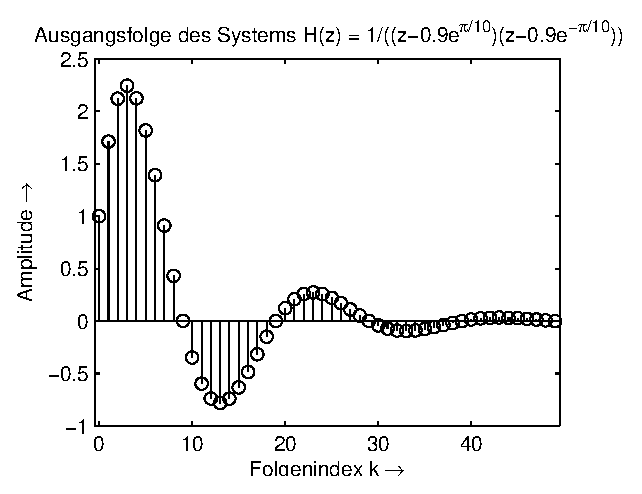
\includegraphics{psZ/BspKonjKomplexPole}
\caption{\label{pic:BspKonjKomplexPol}Beispiel der Impulsantwort eines Systems mit
konjugiert komplexen Polpaar.}
\end{center}
\end{figure}
\hspace{0.1mm}
\end{example}

\section{Stabilität}
Mit den Erklärungen für Abbildung \ref{pic:bspPollagen} ist die
Frage nach einem Stabilitätstest für kausale LTI-Systeme recht einfach zu
beantworten. Da alle Systeme mit Polradien größer eins
aufklingende Schwingungen erzeugen sind die dazugehörigen
Impulsantworten nicht endlich. Auf einen endlichen Impuls reagiert
das System mit einer unendlichen Ausgangsgröße. Damit ist die
BIBO-Bedingung nicht mehr erfüllt.
\wichtig{Stabile, kausale
Systeme haben nur Pole innerhalb des Einheitkreises.}
\wichtig{Quasistabil sind Systeme mit einfachen Polen auf dem Einheitskreis}

Allgemein lässt sich sagen, dass Systeme deren z-Konvergenzgebiet den Einheitskreis
mit einschließen stabil sind. Betrachtet man noch einmal die
Beispiele für z-Transformation und des dazugehörigen Konvergenzgebietes
auf Seite \pageref{Bsp:z_TrafoUndROC}, so wird
deutlich, dass die kausale Folge ein stabiles System darstellt, während die
nicht-kausale Folge instabil ist. Man kann dies auch daran erkennen, dass
die Folge mit wachsendem $k$ größer wird.

Für LTI-Systeme ergibt sich als Kriterium für die BIBO-Stabilität.
\begin{equation}\label{eq:BIBO_INTEGRAL}
    \int_{-\infty}^{\infty} |h(t)|^2 dt < \infty
\end{equation}
bzw. für diskrete Systeme gilt
\begin{equation}\label{eq:BIBO_Diskret}
    \sum_{k = -\infty}^{\infty}|h(k)|^2 < \infty
\end{equation}

\subsection{Stabilität eines Systems 2. Ordnung}
Systeme zweiter Ordnung sind in der digitalen Signalverarbeitung
ein wichtiger Grundbaustein. Es ist deshalb interessant allgemein
die Stabilitätsbedingungen zu berechnen.
Das System ist durch
\begin{equation}
    H(z)=\frac{1}{1+a_{1}z^{-1}+a_{2}z^{-2}}
\end{equation}
gegeben. Um die Polstellen des Polynoms zu berechnen, muss
\begin{equation}
    z^{2}+a_{1}z+a_{2}=0
\end{equation}
\zB mit der bekannten pq-Formel
\begin{eqnarray}
    z_{1}& = &-\frac{a_{1}}{2}+\sqrt{\frac{a_{1}^{2}}{4}-a_{2}}\\
    z_{2}& = &-\frac{a_{1}}{2}-\sqrt{\frac{a_{1}^{2}}{4}-a_{2}}
\end{eqnarray}
berechnet werden.

Die Stabilität ist immer für einen Betrag von $\left|z\right|<1$
gesichert. Welche Bedingungen müssen für die Koeffizienten
$a_1$ und $a_2$ gelten?

Zur Lösung nehmen wir zunächst eine Fallunterscheidung vor:
\begin{enumerate}
    \item{ Für die komplexwertige Lösung $a_{2}>\frac{a_{1}^{2}}{4}$
    ergibt sich durch die Nebenbedingung, dass man $\sqrt{-1} = j$
    vor die Wurzel ziehen kann und sich somit die Vorzeichen umdrehen.
    \begin{equation}
    z=-\frac{a_{1}}{2} \pm j \sqrt{a_{2}-\frac{a_{1}^{2}}{4}}
    \end{equation}
    Berechnet man den Betrag ergibt sich
    \begin{eqnarray}
    \left|z\right| & = & \sqrt{\frac{a_{1}^{2}}{4}+a_{2}-\frac{a_{1}^{2}}{4}}\\
    & = & \sqrt{a_{2}}
    \end{eqnarray}
    Da für ein stabiles System $\left|z\right|<1$ gelten muss, gilt
    als erste Bedingung, dass auch $a^2_{2}<1$ sein muss}

    \item{Für die reelwertige Lösung gilt $a_{2}<\frac{a_{1}^{2}}{4}$:\\
    Es ergibt sich damit die folgende Ungleichung.
    \begin{equation}
        -1 < -\frac{a_{1}}{2} \pm \underbrace{\sqrt{\frac{a_{1}^{2}}{4}-a_{2}}}_{>0} < 1
    \end{equation}
    Löst man diese Ungleichung zunächst für das erste Ungleichheitszeichen und nutzt
    die negative Lösung, da diese ja immer kleiner ist als die positive Lösung
    \begin{equation}
        -1<-\frac{a_{1}}{2} - \sqrt{\frac{a_{1}^{2}}{4}-a_{2}}
    \end{equation}
    ergibt sich (zunächst Multiplikation mit -1, danach quadrieren und ausrechnen)
    \begin{eqnarray}
        -1+\frac{a_{1}}{2} & < & - \sqrt{\frac{a_{1}^{2}}{4}-a_{2}}\\
        \left(1-\frac{a_{1}}{2}\right)^{2}& > & \frac{a_{1}^{2}}{4}-a_{2}\\
        1-2\frac{a_{1}}{2}+\frac{a_{1}^{2}}{4}& > & \frac{a_{1}^{2}}{4}-a_{2}\\
        1-a_1 &  >  & -a_2 \\
        a_{1} & <  & a_{2}+1
    \end{eqnarray}
    Für das zweite Ungleichheitszeichen gilt entsprechendes. Die zweite
    Bedingung lautet
    \begin{equation}\label{eq:SOS:Ungleichung2}
    a_1 > -a_2 -1
    \end{equation}
    }
\end{enumerate}
Fasst man diese Bedingungen zusammen, ergibt sich für $a_2$ eine
untere Grenze von $a_2>-1$.
Alles zusammen beschreibt ein Dreieck, dass als Stabilitätsdreieck
für kausales System 2. Ordnung bezeichnet wird (siehe Abbildung \ref{pic:Stabilddreieck}).

\begin{figure}[H]
\begin{center}
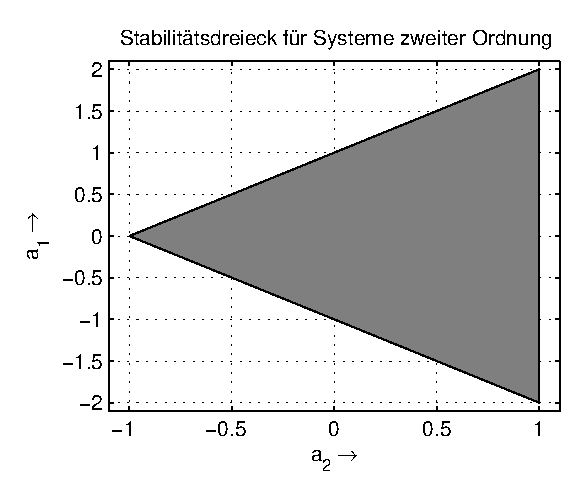
\includegraphics{psZ/Stabildreieck}
\caption{\label{pic:Stabilddreieck}Stabilitätsdreieck für Systeme zweiter Ordnung mit
den Koeffizienten $a_1$ und $a_2$.}
\end{center}
\end{figure}
\compileif{bBook}
{
\section{Matlab und z-Transformation}
\tbd{poly roots Anwendung erklären\\ zplane als Anzeige Tool }

}

\section{Übungen}
\subsection{Wiederholung des Stoffes und einfache Rechenaufgaben}
\begin{enumerate}
    \item Welche Bedingungen müssen gelten, damit ein LTI-System stabil ist?
    \item Welche Beschreibungen eines LTI-Systems kennen Sie?
    \item Warum ist die Angabe der z-Transformationsfunktion nicht ausreichend?
    \item \label{Aufg:zTrafo:Stabilitaet}Testen Sie die folgenden LTI - Systeme auf Stabilität:
    \begin{enumerate}
        \item $y(k) = -2 y(k-1) + 1.5 x(k) - 2x(k-1)$
        \item $y(k) =  2.5 x(k-1) + 1.83 y(k-1)  - 0.99y(k-2)$
        \item $y(k) =  0.3 x(k) + 07 x(k-1) + 1.9812 y(k-1)   - 1.0201 y(k-2)$
    \end{enumerate}
    \item{Zeigen Sie, dass die Ungleichung \ref{eq:SOS:Ungleichung2} gilt.}
\end{enumerate}
\subsection{Aufgaben (Auf Klausurniveau)\label{Aufg:zTrafo:Klausurniveau}}
\begin{enumerate}
    \item Zeigen Sie, dass die z-Transformation eine lineare Transformation ist, indem
    Sie den Linearitätstest durchführen.
    \item \label{Aufg:zTrafo:zTrafo}Welchen Wert hat das folgende System nach 50 Schritten. Geben Sie die direkte
    Berechnungsmethode an. Ist das System BIBO-stabil?\\
    $y(k) = \sqrt(2) y(k-1) -  y(k-2) + 0.5 \delta(k)$
    \item Sind die folgenden Systeme kausal, stabil, linear und
    zeitinvariant? Begründen Sie ihre Antwort (auch wenn Sie keine Aussage machen können) mathematisch oder
    textuell (16)!
    \begin{enumerate}
        \item $y(k) = 0.5 y(k-1) - 0.3 y(k-2) k + 0.4 x(k) - 0.5
        x(k-1)x(k-2)$
        \item $y(k+1) = 1.1 y(k-1) - 0.5 x(k+1) + 0.3 x(k) - 0.5
        x(k-1)$
        \item $y(k+1) = 2x(2k-k) - y(k+1) + 4 x(k-2) + 1.8 y(k-1)$
        \item $y(k) = 0.3 x(k) + 0.6x(k-1) - 0.7 x(k-2)y(k-2) + x(2k-2)$
    \end{enumerate}
    \item Ist das folgende Systeme kausal, stabil, linear und
    zeitinvariant? Begründen Sie ihre Antwort mathematisch oder
    textuell! Falls Sie keine Aussage treffen können, begründen Sie auch dies!
    $y(k+1) - 2y(k+2) + \alpha x(k+2) + x(k+1) =  1.99 y(k)$\\
    Nehmen Sie an $\alpha = 2$ (8 Punkte). Für welche Bereiche von $\alpha$ (rein reell)
    ist das System stabil (Begründung)? (2 Punkte)
    \item Sind die beiden folgenden Systeme kausal, stabil, linear und
    zeitinvariant? Begründen Sie ihre Antwort mathematisch oder
    textuell! Falls Sie keine Aussage treffen können, begründen Sie auch dies!
    \begin{enumerate}
    \item $y(k) + \beta^2 y(k-2) + x(k-2) = 2 x(k) - 2x(k-2) - 1.9
    y(k-1)$.\\
    Zur Beantwortung der Frage nehmen Sie an $\beta = \sqrt{0.5}$ (8 Punkte).\\
    Für welche Bereiche von $\beta$ ist das System stabil bzw.
    instabil (4 Punkte).
    \item $2y(k) - 3.7x(-k-2)k -0.3y(k-3) = 10x(k-10)$. (8 Punkte)
    \end{enumerate}

\end{enumerate}

\compileif{bBook}
{
\subsection{Matlab-Aufgaben}
\begin{enumerate}
    \item Lösen Sie die Aufgabe \ref{Aufg:zTrafo:Klausurniveau}.\ref{Aufg:zTrafo:zTrafo} durch
    den Aufbau des Systems und Iteration.
    \item Programmieren Sie eine Funktion, die einen Pol-Nullstellenplan zeichnet und zusätzlich im
    Titel den $b_0$-Koeffizienten ausgibt. Nutzen Sie als Anhaltspunkt die {\tt zplane} Funktion von Matlab.
    Hinweis: Sie benötigen den {\tt axis} Befehl um eine quadratische Grafik aufzubauen (siehe help).
    Sie sollten die {\tt mpoles} Funktion nutzen, um Mehrfach Null- bzw. Polstellen herauszufinden.
    \item Schreiben Sie eine Funktion, die es ermöglicht Systeme durch eine grafische Eingabe mit der Maus
    zu definieren. Zeichnen Sie dazu den Einheitskreis in eine figure. Hinweis: Sie benötigen den
    {\tt ginput} Befehl für die Maus-Eingabe und {\tt axis}, um eine quadratische Grafik zu erzeugen.
\end{enumerate}
}
\subsection{Transfer-Leistung}
\begin{enumerate}
    \item Wie sieht das Konvergenzgebiet für endliche Folgen aus?
    \item
    \item
\end{enumerate}
%
\compileif{bZusammenfassung}
{
\section{Zusammenfassung}
Die wichtigen Erkenntnisse aus diesem Kapitel sind:
\begin{itemize}
    \item Die Systemfunktion ist eine vollständige Beschreibung eines LTI-Systems
    \item Die Systemfunktion ist die z-Transformierte der Impulsantwort
    \item Die Angabe der z-Transformation ist nur mit ROC vollständig.
    \item Das Pol-Nullstellendiagramm ist bis auf die Grundverstärkung $b_0$ eine
    vollständige Beschreibung eines LTI-Systems
    \item Die Stabilität eines kausalen LTI-Systems lässt sich
in der z-Ebene durch die Berechnung der Polradien einfach testen. Es muss gelten, dass
alle Radien kleiner eins sind. Für strikt nicht-kausale Systeme müssen alle Radien größer eins sein, um
ein stabiles System darzustellen.
    \item Bei Systemen zweiter Ordnung müssen um stabile kausale Systeme zu realisieren,
    die rekursiven Koeffizienten $a_1$ und $a_2$ im
    Stabilitätsdreieck liegen.
    \item Pol- bzw. Nullstellen reeller Systeme sind entweder reellwertig oder treten als
    konjugiert komplexe Polpaare auf.
\end{itemize}

}
%\section{Lösungen zu den Aufgaben}
%\subsection{Wiederholung des Stoffes und einfache Rechenaufgaben}
%\begin{enumerate}
%    \item Welche Bedingungen müssen gelten, damit ein LTI-System stabil ist?
%    \loesung{Für kausale Systeme müssen alle Polradien innerhalb des Einheitskreises liegen.}
%    \item Welche Beschreibungen eines LTI-Systems kennen Sie?
%    \loesung{Vollständige Beschreibungen sind: Differenzengleichung, Systemfunktion, Impulsantwort}
%    \item Warum ist die Angabe der z-Transformationsfunktion nicht ausreichend?
%    \loesung{Untescheidliche Folgen haben die gleiche z-Transformierte.}
%    \item \label{Aufg:zTrafo:Stabilitaet}Testen Sie die folgenden LTI - Systeme auf Stabilität:
%    \begin{enumerate}
%        \item $y(k) = -2 y(k-1) + 1.5 x(k) - 2x(k-1)$
%        \loesung{Nicht Stabil, Pol außerhalb}
%        \item $y(k) =  2.5 x(k-1) + 1.83 y(k-1)  - 0.99y(k-2)$
%        \loesung{stabil, siehe Stabilitätsdreieck}
%        \item $y(k) =  0.3 x(k) + 07 x(k-1) + 1.9812 y(k-1)   - 1.0201 y(k-2)$
%        \loesung{instabil, siehe Stabilitätsdreieck}
%    \end{enumerate}
%\end{enumerate}
%\subsection{Aufgaben (Auf Klausurniveau)\label{Aufg:zTrafo:Klausurniveau}}
%\begin{enumerate}
%    \item Zeigen Sie, dass die z-Transformation eine lineare Transformation ist, indem
%    Sie den Linearitätstest durchführen.
%    \loesung{Hmmm}
%    \item \label{Aufg:zTrafo:zTrafo}Welchen Wert hat das folgende System nach 50 Schritten. Geben Sie die direkte
%    Berechnungsmethode an. Ist das System BIBO-stabil?\\
%    $y(k) = \sqrt(2) y(k-1) -  y(k-2) + 0.5 \delta(k)$
%    \item Sind die folgenden Systeme kausal, stabil, linear und
%    zeitinvariant? Begründen Sie ihre Antwort (auch wenn Sie keine Aussage machen können) mathematisch oder
%    textuell (16)!
%    \begin{enumerate}
%        \item $y(k) = 0.5 y(k-1) - 0.3 y(k-2) k + 0.4 x(k) - 0.5
%        x(k-1)x(k-2)$
%        \item $y(k+1) = 1.1 y(k-1) - 0.5 x(k+1) + 0.3 x(k) - 0.5
%        x(k-1)$
%        \item $y(k+1) = 2x(2k-k) - y(k+1) + 4 x(k-2) + 1.8 y(k-1)$
%        \item $y(k) = 0.3 x(k) + 0.6x(k-1) - 0.7 x(k-2)y(k-2) + x(2k-2)$
%    \end{enumerate}
%    \item Ist das folgende Systeme kausal, stabil, linear und
%    zeitinvariant? Begründen Sie ihre Antwort mathematisch oder
%    textuell! Falls Sie keine Aussage treffen können, begründen Sie auch dies!
%    $y(k+1) - 2y(k+2) + \alpha x(k+2) + x(k+1) =  1.99 y(k)$\\
%    Nehmen Sie an $\alpha = 2$ (8 Punkte). Für welche Bereiche von $\alpha$ (rein reell)
%    ist das System stabil (Begründung)? (2 Punkte)
%    \item Sind die beiden folgenden Systeme kausal, stabil, linear und
%    zeitinvariant? Begründen Sie ihre Antwort mathematisch oder
%    textuell! Falls Sie keine Aussage treffen können, begründen Sie auch dies!
%    \begin{enumerate}
%    \item $y(k) + \beta^2 y(k-2) + x(k-2) = 2 x(k) - 2x(k-2) - 1.9
%    y(k-1)$.\\
%    Zur Beantwortung der Frage nehmen Sie an $\beta = \sqrt{0.5}$ (8 Punkte).\\
%    Für welche Bereiche von $\beta$ ist das System stabil bzw.
%    instabil (4 Punkte).
%    \item $2y(k) - 3.7x(-k-2)k -0.3y(k-3) = 10x(k-10)$. (8 Punkte)
%    \end{enumerate}
%
%\end{enumerate}
%
%\subsection{Matlab-Aufgaben}
%\begin{enumerate}
%    \item Lösen Sie die Aufgabe \ref{Aufg:zTrafo:Klausurniveau}.\ref{Aufg:zTrafo:zTrafo} durch
%    den Aufbau des Systems und Iteration.
%    \item Programmieren Sie eine Funktion, die einen Pol-Nullstellenplan zeichnet und zusätzlich im
%    Titel den $b_0$-Koeffizienten ausgibt. Nutzen Sie als Anhaltspunkt die \verb/zplane/ Funktion von Matlab.
%    Hinweis: Sie benötigen den \verb/axis/ Befehl um eine quadratische Grafik aufzubauen (siehe help).
%    Sie sollten die \verb/mpoles/ Funktion nutzen, um Mehrfach Null- bzw. Polstellen herauszufinden.
%    \item Schreiben Sie eine Funktion, die es ermöglicht Systeme durch eine grafische Eingabe mit der Maus
%    zu definieren. Zeichnen Sie dazu den Einheitskreis in eine figure. Hinweis: Sie benötigen den
%    \verb/ginput/ Befehl für die Maus-Eingabe und \verb/axis/, um eine quadratische Grafik zu erzeugen.
%\end{enumerate}
%
%\subsection{Transfer-Leistung}
%\begin{enumerate}
%    \item Wie sieht das Konvergenzgebiet für endliche Folgen aus?
%    \item
%    \item
%\end{enumerate}
